\documentclass[a4paper,11pt]{article}
\usepackage{pgfplots}
\usepackage{siunitx}
\sisetup{detect-weight,exponent-product=\cdot,output-decimal-marker={,},
	per-mode=symbol,binary-units=true,range-phrase={-},range-units=single}
\SendSettingsToPgf
\usetikzlibrary{pgfplots.groupplots}
\pgfplotsset{compat=1.11}
\usepgfplotslibrary{external}
\tikzexternalize

\textwidth 160mm \textheight 247mm

\pgfplotsset{width=\figurewidth,compat=1.11}
\pgfplotsset{
	tick label style={font=\tiny},
	label style={font=\footnotesize},
	legend style={font=\footnotesize},
	title style={font=\footnotesize}
}


\newcommand{\szer}{16cm}
\newcommand{\wys}{5.6cm}
\newcommand{\odstepionowy}{1.2cm}


\begin{document}

\tikzsetnextfilename{}

\begin{figure}[Odpowiedź skokowa toru u1 - y1]
\tikzsetnextfilename{zad2_u1y1}
\begin{tikzpicture}
\begin{groupplot}[group style={group size=1 by 2,vertical sep=\odstepionowy},
width=\szer,height=\wys]
%%1
\nextgroupplot
[xmin=1,xmax=300,ymin=-2.5,ymax=2.5,
xtick={0,50,...,300},
ytick={-2.5,-2,...,4},
ylabel={$y_1(k)$},
xlabel={$k$}]
\addplot[const plot,color=blue,semithick] file {datadir/zad2/skok_sterowania_u1_y1/wyjscie_y1_u1_skok_-0.8.txt};
\addplot[const plot,color=red,semithick] file {datadir/zad2/skok_sterowania_u1_y1/wyjscie_y1_u1_skok_-0.4.txt};
\addplot[const plot,color=green,semithick] file {datadir/zad2/skok_sterowania_u1_y1/wyjscie_y1_u1_skok_0.4.txt};
\addplot[const plot,color=purple,semithick] file {datadir/zad2/skok_sterowania_u1_y1/wyjscie_y1_u1_skok_0.8.txt};
\nextgroupplot
%%2
[xmin=1,xmax=300,ymin=-1.5,ymax=1.5,
xtick={0,50,...,300},
ytick={-2.5,-2,...,4},
ylabel={$u_1(k)$},
xlabel={$k$}]
\addplot[const plot,color=blue,semithick] file {datadir/zad2/skok_sterowania_u1_y1/sterowanie1_y1_skok_-0.8.txt};
\addplot[const plot,color=red,semithick] file {datadir/zad2/skok_sterowania_u1_y1/sterowanie1_y1_skok_-0.4.txt};
\addplot[const plot,color=green,semithick] file {datadir/zad2/skok_sterowania_u1_y1/sterowanie1_y1_skok_0.4.txt};
\addplot[const plot,color=purple,semithick] file {datadir/zad2/skok_sterowania_u1_y1/sterowanie1_y1_skok_0.8.txt};
\end{groupplot}
\end{tikzpicture}
\end{figure}

\begin{figure}[Odpowiedź skokowa toru u1 - y2]
\tikzsetnextfilename{zad2_u1y2}
\begin{tikzpicture}
\begin{groupplot}[group style={group size=1 by 2,vertical sep=\odstepionowy},
width=\szer,height=\wys]
%%1
\nextgroupplot
[xmin=1,xmax=300,ymin=-2.5,ymax=2.5,
xtick={0,50,...,300},
ytick={-2.5,-2,...,4},
ylabel={$y_2(k)$},
xlabel={$k$}]
\addplot[const plot,color=blue,semithick] file {datadir/zad2/skok_sterowania_u1_y2/wyjscie_y2_u1_skok_-0.8.txt};
\addplot[const plot,color=red,semithick] file {datadir/zad2/skok_sterowania_u1_y2/wyjscie_y2_u1_skok_-0.4.txt};
\addplot[const plot,color=green,semithick] file {datadir/zad2/skok_sterowania_u1_y2/wyjscie_y2_u1_skok_0.4.txt};
\addplot[const plot,color=purple,semithick] file {datadir/zad2/skok_sterowania_u1_y2/wyjscie_y2_u1_skok_0.8.txt};
\nextgroupplot
%%2
[xmin=1,xmax=300,ymin=-1.5,ymax=1.5,
xtick={0,50,...,300},
ytick={-2.5,-2,...,4},
ylabel={$u_1(k)$},
xlabel={$k$}]
\addplot[const plot,color=blue,semithick] file {datadir/zad2/skok_sterowania_u1_y2/sterowanie1_y2_skok_-0.8.txt};
\addplot[const plot,color=red,semithick] file {datadir/zad2/skok_sterowania_u1_y2/sterowanie1_y2_skok_-0.4.txt};
\addplot[const plot,color=green,semithick] file {datadir/zad2/skok_sterowania_u1_y2/sterowanie1_y2_skok_0.4.txt};
\addplot[const plot,color=purple,semithick] file {datadir/zad2/skok_sterowania_u1_y2/sterowanie1_y2_skok_0.8.txt};
\end{groupplot}
\end{tikzpicture}
\end{figure}


\begin{figure}[Odpowiedź skokowa toru u2 - y1]
\tikzsetnextfilename{zad2_u2y1}
\begin{tikzpicture}
\begin{groupplot}[group style={group size=1 by 2,vertical sep=\odstepionowy},
width=\szer,height=\wys]
%%1
\nextgroupplot
[xmin=1,xmax=300,ymin=-2.5,ymax=2.5,
xtick={0,50,...,300},
ytick={-2.5,-2,...,4},
ylabel={$y_1(k)$},
xlabel={$k$}]
\addplot[const plot,color=blue,semithick] file {datadir/zad2/skok_sterowania_u2_y1/wyjscie_y1_u2_skok_-0.8.txt};
\addplot[const plot,color=red,semithick] file {datadir/zad2/skok_sterowania_u2_y1/wyjscie_y1_u2_skok_-0.4.txt};
\addplot[const plot,color=green,semithick] file {datadir/zad2/skok_sterowania_u2_y1/wyjscie_y1_u2_skok_0.4.txt};
\addplot[const plot,color=purple,semithick] file {datadir/zad2/skok_sterowania_u2_y1/wyjscie_y1_u2_skok_0.8.txt};
\nextgroupplot
%%2
[xmin=1,xmax=300,ymin=-1.5,ymax=1.5,
xtick={0,50,...,300},
ytick={-2.5,-2,...,4},
ylabel={$u_2(k)$},
xlabel={$k$}]
\addplot[const plot,color=blue,semithick] file {datadir/zad2/skok_sterowania_u2_y1/sterowanie2_y1_skok_-0.8.txt};
\addplot[const plot,color=red,semithick] file {datadir/zad2/skok_sterowania_u2_y1/sterowanie2_y1_skok_-0.4.txt};
\addplot[const plot,color=green,semithick] file {datadir/zad2/skok_sterowania_u2_y1/sterowanie2_y1_skok_0.4.txt};
\addplot[const plot,color=purple,semithick] file {datadir/zad2/skok_sterowania_u2_y1/sterowanie2_y1_skok_0.8.txt};
\end{groupplot}
\end{tikzpicture}
\end{figure}

\begin{figure}[Odpowiedź skokowa toru u2 - y2]
\tikzsetnextfilename{zad2_u2y2}
\begin{tikzpicture}
\begin{groupplot}[group style={group size=1 by 2,vertical sep=\odstepionowy},
width=\szer,height=\wys]
%%1
\nextgroupplot
[xmin=1,xmax=300,ymin=-2.5,ymax=2.5,
xtick={0,50,...,300},
ytick={-2.5,-2,...,4},
ylabel={$y_2(k)$},
xlabel={$k$}]
\addplot[const plot,color=blue,semithick] file {datadir/zad2/skok_sterowania_u2_y2/wyjscie_y2_u2_skok_-0.8.txt};
\addplot[const plot,color=red,semithick] file {datadir/zad2/skok_sterowania_u2_y2/wyjscie_y2_u2_skok_-0.4.txt};
\addplot[const plot,color=green,semithick] file {datadir/zad2/skok_sterowania_u2_y2/wyjscie_y2_u2_skok_0.4.txt};
\addplot[const plot,color=purple,semithick] file {datadir/zad2/skok_sterowania_u2_y2/wyjscie_y2_u2_skok_0.8.txt};
\nextgroupplot
%%2
[xmin=1,xmax=300,ymin=-1.5,ymax=1.5,
xtick={0,50,...,300},
ytick={-2.5,-2,...,4},
ylabel={$u_2(k)$},
xlabel={$k$}]
\addplot[const plot,color=blue,semithick] file {datadir/zad2/skok_sterowania_u2_y2/sterowanie2_y2_skok_-0.8.txt};
\addplot[const plot,color=red,semithick] file {datadir/zad2/skok_sterowania_u2_y2/sterowanie2_y2_skok_-0.4.txt};
\addplot[const plot,color=green,semithick] file {datadir/zad2/skok_sterowania_u2_y2/sterowanie2_y2_skok_0.4.txt};
\addplot[const plot,color=purple,semithick] file {datadir/zad2/skok_sterowania_u2_y2/sterowanie2_y2_skok_0.8.txt};
\end{groupplot}
\end{tikzpicture}
\end{figure}


\begin{figure}[Charakterystyka statyczna]
\tikzsetnextfilename{zad2_charstat}
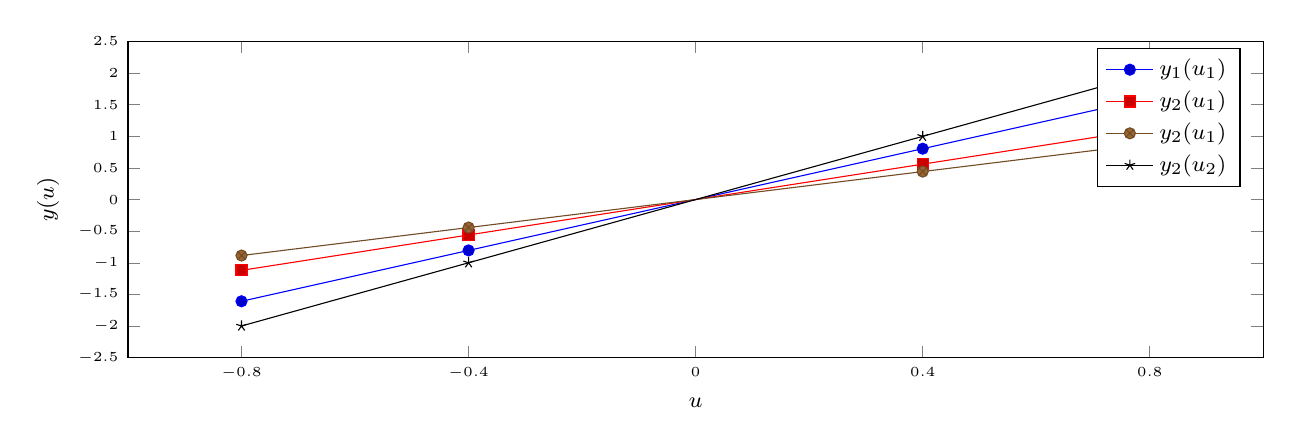
\begin{tikzpicture}
\begin{groupplot}[group style={group size=1 by 2,vertical sep=\odstepionowy},
width=\szer,height=\wys]
%%1
\nextgroupplot
[xmin=-1,xmax=1,ymin=-2.5,ymax=2.5,
xtick={-0.8, -0.4, 0, 0.4, 0.8},
ytick={-2.5,-2,...,2.5},
ylabel={$y(u)$},
xlabel={$u$}]
    \addplot coordinates { (-0.8,-1.607363) (-0.4,-8.036813e-01) (0.4,8.036813e-01) (0.8,1.607363) }; 
    \addplot coordinates { (-0.8,-1.118859) (-0.4,-5.594296e-01) (0.4,5.594296e-01) (0.8,1.118859) }; 
    \addplot coordinates { (-0.8,-0.884545) (-0.4,-4.422727e-01) (0.4,4.422727e-01) (0.8,0.884545) }; 
    \addplot coordinates { (-0.8,-1.997861) (-0.4,-9.989305e-01) (0.4,9.989305e-01) (0.8,1.997861) }; 
	\legend{ $y_1(u_1)$, $y_2(u_1)$, $y_2(u_1)$, $y_2(u_2)$ }
\end{groupplot}
\end{tikzpicture}
\end{figure}

\end{document}
